\paragraph{Battle for Middle Earth}

\subparagraph{Outline}

4x4, neutrals 2/4, wastelands 10/10, base: +5.

No rf, no OP, no OD, just blockade card. Cards are seen through the fog -> Can't blockade a bottleneck to trap armies (see \href{https://www.warzone.com/MultiPlayer?GameID=29950732}{Mori's POV T19} or \href{https://www.warzone.com/MultiPlayer?GameID=39987378}{Timi's POV T5}). No RF -> No rush for card piece.


\subparagraph{Map Dynamics}

\begin{itemize}
    \item The map is essentially divided into compartments, reflecting its LOTR theme. This includes West and East, separated by the river Anduin (iirc). There are only 3 routes between West and East, and all are quite slow, which means it's preferable to have picks in both areas. 
    \item West more Income than East. West > East. In some distributions, you might completely ignore the East, especially if it has too many wastelands. However, this is a rare occurrence.
\end{itemize}

For what is worth (I don't think it is whatsoever), the WR for the only bonuses you should care about at Figure \ref{bfme_wr}. 

\begin{figure}[H]
  \centering
  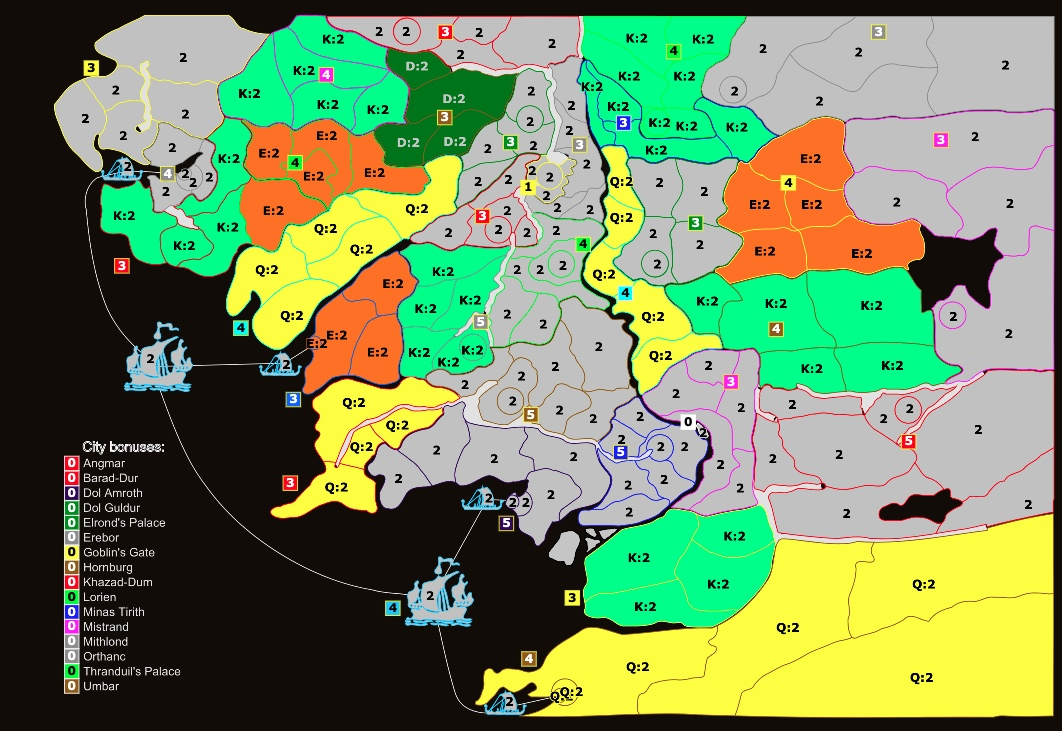
\includegraphics[width=0.9\textwidth]{Images/bfme.jpg}
  \caption{Bonus Win Rates for Games with Overall Winner Rating >=1800 in BFME(n=378) (D>K>Q>E>-).}
  \label{bfme_wr}
\end{figure}

\subparagraph{Gameplay}

Due to how the map is divided, position >>>> income. Especially when considering a) it's RMO and b) you can see the blocakdes, you really are better of picking like \href{https://www.warzone.com/MultiPlayer?GameID=41216429}{here} with a simple 1/2/4 East and cover pick West and a gamelan of getting to 12 Income, building a stack and deleting everything in the West.
\\
\\
A good 9/10 games involves the same ten bonuses and their FTBs and rarely their expansion. Since there is no rf card, you aren't forced to expand / take a risk losing armies to neutrals. This can lead to positions such as \href{https://www.warzone.com/MultiPlayer?GameID=38352157}{this 71 Turn long game} where both players just can't find a way in. You can see that the players don't pick for Income progression, rather position. The board has a +4 FTB west, a safe +3 in Enedwaith and a contested cluster east. Muli covers the board with 1/2 East to secure coverage, 3 on the safe +3 bonus, 4/5/6/7 on the +4 FTB and 8 to combo with 1 for combinations like 1/3/7/8. $\text{Jacoþ thε Restle§°ⁿ³}$ has 1/2/3 west, 4/5/6/7 for east coverage and 8 West. It's actually a really funny game, I wish it was mine and I had an account to favorite it.
\\
\\
Instead of checking games with specific distributions, here's some games with weird picks so we can laugh and forget how bad this template is:
\begin{itemize}
    \item Dunland (Grey +5) is and isn't a great pick. It is however great to expand to in distributions that aren't 1/2 +3 ftb 3/4/5/6 +4 ftb 7/8 cover, such as \href{https://www.warzone.com/MultiPlayer?GameID=41315344}{here by Aika}. You can surely combo it like \href{https://www.warzone.com/MultiPlayer?GameID=38140304}{here by Octane}, \href{https://www.warzone.com/MultiPlayer?GameID=40139613}{here by Aika} and finally \href{https://www.warzone.com/MultiPlayer?GameID=33355814}{again by Octane}. And you can of course use it to combo the +3 for an FTB.
    \item Rohan is nice to expand into as the West vs East player, but to pick it you have to be brave like \href{https://www.warzone.com/MultiPlayer?GameID=38695939}{Malakkan} or \href{https://www.warzone.com/MultiPlayer?GameID=33861437}{Bechaa} (and still lose)
    \item I respect everyone who picks East Gondor but it ain't it. In fact, mini-game time for you viewer. The games below are between 1800 Rated + players and the East Gondor player won only once, but it's up to you to find out which link is correct. \href{https://www.warzone.com/MultiPlayer?GameID=36755511}{Example 1}, \href{https://www.warzone.com/MultiPlayer?GameID=36668057}{Example 2}, \href{https://www.warzone.com/MultiPlayer?GameID=29914718}{Example 3}, \href{https://www.warzone.com/MultiPlayer?GameID=25557005}{Example 4}, \href{https://www.warzone.com/MultiPlayer?GameID=16951613}{Example 5} and \href{https://www.warzone.com/MultiPlayer?GameID=15253205}{Example 6}.
\end{itemize}
